% ============================================================================
%  The Multidimensional Geometry of Truth in LLMs 
%  Author: Ilyass Ouardi  -
%  Universita degli Studi di Milano
%
%  AUTHOR VOICE CONVENTION:
%    * "I"  — methodological choices, engineering decisions
%    * "We" — inclusive mathematical exposition only
% ============================================================================

\documentclass[sn-basic]{sn-jnl}

% Packages -------------------------------------------------------------------
\usepackage[utf8]{inputenc}
\usepackage[T1]{fontenc}
\usepackage{lmodern}
\usepackage{microtype}
\usepackage{textcomp}

\usepackage[title]{appendix}
\usepackage{manyfoot}

\usepackage{amsmath, amssymb, amsthm, amsfonts}
\usepackage{mathrsfs}

\usepackage{graphicx}
\usepackage{xcolor}
\usepackage{colortbl}

\usepackage{tikz}
\usetikzlibrary{positioning, arrows.meta, fit, shapes.geometric, calc}
\usepackage{pgfplots}
\pgfplotsset{compat=1.18}

\usepackage{booktabs}
\usepackage{multirow}
\usepackage{enumitem}

\usepackage{algorithm}
\usepackage{algorithmicx}
\usepackage{algpseudocode}
\usepackage{listings}

\usepackage{url}
\usepackage{hyperref}
\hypersetup{ colorlinks=true, linkcolor=blue!50!black, citecolor=blue!50!black,
    urlcolor=blue!50!black }

\usepackage{cleveref}

% Color macros for tables
\definecolor{bestcolor}{HTML}{C62828}
\definecolor{secondcolor}{HTML}{1565C0}
\definecolor{failcolor}{HTML}{FFCDD2}
\definecolor{passcolor}{HTML}{C8E6C9}
\newcommand{\best}[1]{\textcolor{bestcolor}{\textbf{#1}}}
\newcommand{\second}[1]{\textcolor{secondcolor}{\underline{#1}}}

% Definition environment
\newtheorem{definition}{Definition}[section]

% Working notations ----------------------------------------------------------
\newcommand{\bmu}{\boldsymbol{\mu}} \newcommand{\bnu}{\boldsymbol{\nu}}
\newcommand{\dimv}{\theta_{\text{DIM}}}
\newcommand{\fablate}[1][\cdot]{f_{\text{ablate}(#1)}}
\newcommand{\fadd}[1][\cdot]{f_{\text{add}(#1,\alpha)}}
\newcommand{\Labl}{\mathcal{L}_{\text{abl}}}
\newcommand{\Ladd}{\mathcal{L}_{\text{add}}}
\newcommand{\Lret}{\mathcal{L}_{\text{ret}}}

\begin{document}

\title[Truth as a Concept Cone]{The Multidimensional Geometry of Truth in Large Language Models: A Concept-Cone Extension of the Linear Representation Hypothesis}

\author[1]{\fnm{Ilyass} \sur{Ouardi}}\email{ilyass.ouardi@studenti.unimi.it}

\affil[1]{\orgdiv{Department of Computer Science}, \orgname{Universit\`a degli
Studi di Milano}, \city{Milan}, \country{Italy}}

\date{\today}


% ============================================================================
%  ABSTRACT
% ============================================================================



\abstract{ The Linear Representation Hypothesis holds that high-level concepts
are encoded as linear directions in a language model's residual stream. Under
this hypothesis, propositional truth is modeled as one such direction: a
Difference-in-Means (DIM) probe recovers it, and adding or ablating that
direction can flip the model's True/False verdict. Recent work on refusal
suggests this single direction may be the one-dimensional case of a
multi-dimensional \emph{concept cone}, a linear subspace whose interior mediates
the behaviour. This project asks whether truth has the same structure. I test
two methods: \emph{Truth Direction Optimization} (TDO), a gradient-based
refinement of the DIM direction under a loss that encodes two causal axioms and
a KL-retention term; and \emph{Truth Cone Optimization} (TCO), which extends
this to a $k$-dimensional orthonormal cone and, at every step, samples
directions from \emph{inside} the cone so the optimizer targets the interior
rather than only the basis. On six instruction-tuned models from three families
(Qwen-2.5 1.5/7/14B, Gemma-2 2/9B, Llama-3.1-8B), a single direction is causally
sufficient for the smaller models but fails for the larger ones on two axes at
once: low ablation Answer Switching Rate and raised KL divergence on unrelated
prompts. A $2$-D cone closes both gaps for every model. The basis vectors are
near-orthogonal to the DIM probe ($|\cos| < 0.1$) yet each is individually
causally effective. For the models I tested, this is consistent with truth
occupying a small multi-dimensional linear subspace rather than a single line. }


\maketitle

% ============================================================================
%  Figure 1 — Teaser (Step 6 of paper-writing workflow)
%  ----------------------------------------------------------------------------
%  Two-panel headline figure. Left: mean MC ASR vs cone dim k.
%  Right: mean KL retention vs k, with surgicality threshold 0.1.
%  Same color per model across both panels.
%
%  Required packages:
%     \usepackage{pgfplots}
%     \pgfplotsset{compat=1.18}
%     \usepackage{xcolor}
%
%  Data is hard-coded from results_summary.json (Exp 3 and Exp 5).
% ============================================================================

\begin{figure}[t]
\centering
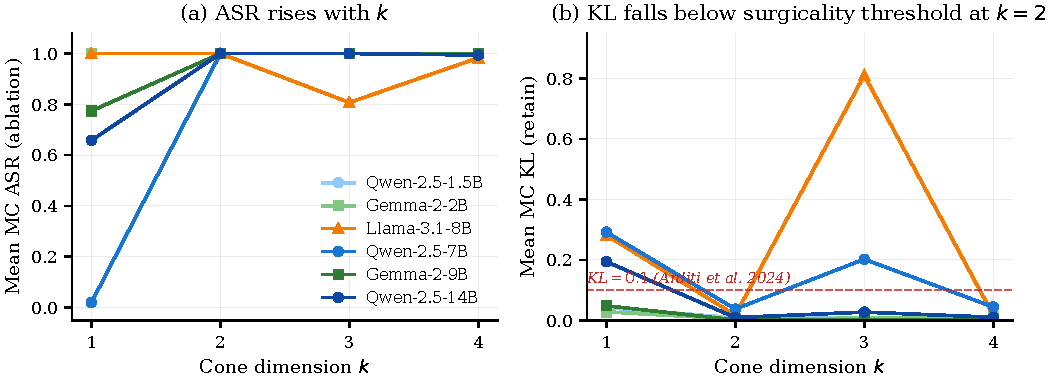
\includegraphics[width=\linewidth]{figures/fig_teaser.pdf}
% \definecolor{qw15}{HTML}{90CAF9}   % qwen-2.5-1.5b   light blue
% \definecolor{qw7}{HTML}{1976D2}    % qwen-2.5-7b     mid blue
% \definecolor{qw14}{HTML}{0D47A1}   % qwen-2.5-14b    deep blue
% \definecolor{gm2}{HTML}{81C784}    % gemma-2-2b      light green
% \definecolor{gm9}{HTML}{2E7D32}    % gemma-2-9b      deep green
% \definecolor{ll8}{HTML}{F57C00}    % llama-3.1-8b    orange
% \definecolor{thresholdred}{HTML}{C62828}

% \begin{tikzpicture}

% % --- LEFT PANEL: mean MC ASR (in-distribution, ablation) vs k ---------------
% \begin{axis}[
%     name=asrplot,
%     width=0.50\linewidth, height=5.5cm,
%     xlabel={Cone dimension $k$},
%     ylabel={Mean MC ASR (ablation)},
%     xmin=0.8, xmax=4.2,
%     ymin=-0.05, ymax=1.10,
%     xtick={1,2,3,4},
%     ytick={0, 0.25, 0.5, 0.75, 1.0},
%     grid=both, grid style={gray!20, line width=0.3pt},
%     legend style={font=\scriptsize, at={(0.55,0.36)}, anchor=north,
%                   draw=gray!50, fill=white, fill opacity=0.85,
%                   text opacity=1, row sep=-2pt},
%     legend cell align=left,
%     tick label style={font=\scriptsize},
%     label style={font=\small},
%     title={\small \textbf{(a)} ASR rises with $k$},
%     title style={yshift=-1ex},
%     every axis plot/.append style={line width=0.9pt, mark size=2pt}
% ]

% % qwen-2.5-1.5b
% \addplot[color=qw15, mark=*]        coordinates {(1,1.000)(2,1.000)(3,1.000)(4,1.000)};
% % gemma-2-2b
% \addplot[color=gm2, mark=square*]   coordinates {(1,1.000)(2,1.000)(3,1.000)(4,1.000)};
% % llama-3.1-8b
% \addplot[color=ll8, mark=triangle*] coordinates {(1,1.000)(2,1.000)(3,0.807)(4,0.983)};
% % qwen-2.5-7b
% \addplot[color=qw7, mark=*]         coordinates {(1,0.020)(2,1.000)(3,1.000)(4,1.000)};
% % gemma-2-9b
% \addplot[color=gm9, mark=square*]   coordinates {(1,0.774)(2,1.000)(3,1.000)(4,1.000)};
% % qwen-2.5-14b
% \addplot[color=qw14, mark=*]        coordinates {(1,0.658)(2,1.000)(3,1.000)(4,0.994)};

% \legend{Qwen-2.5-1.5B, Gemma-2-2B, Llama-3.1-8B,
%         Qwen-2.5-7B, Gemma-2-9B, Qwen-2.5-14B}
% \end{axis}


% % --- RIGHT PANEL: mean MC KL on retain set vs k -----------------------------
% \begin{axis}[
%     at={($(asrplot.east) + (1.4cm,0)$)}, anchor=west,
%     width=0.50\linewidth, height=5.5cm,
%     xlabel={Cone dimension $k$},
%     ylabel={Mean MC KL (retain)},
%     xmin=0.8, xmax=4.2,
%     ymin=0, ymax=0.95,
%     xtick={1,2,3,4},
%     ytick={0, 0.1, 0.25, 0.5, 0.75},
%     extra y ticks={0.1},
%     extra y tick labels={},
%     extra y tick style={grid=major, grid style={thresholdred, dashed, line width=0.8pt}},
%     grid=both, grid style={gray!20, line width=0.3pt},
%     tick label style={font=\scriptsize},
%     label style={font=\small},
%     title={\small \textbf{(b)} KL falls below surgicality threshold at $k{=}2$},
%     title style={yshift=-1ex},
%     every axis plot/.append style={line width=0.9pt, mark size=2pt}
% ]

% % Threshold callout
% \node[font=\scriptsize\itshape, text=thresholdred, anchor=west]
%     at (axis cs:0.85, 0.135) {KL $= 0.1$ (Arditi et al.~2024)};

% % qwen-2.5-1.5b
% \addplot[color=qw15, mark=*]        coordinates {(1,0.042)(2,0.008)(3,0.009)(4,0.008)};
% % gemma-2-2b
% \addplot[color=gm2,  mark=square*]  coordinates {(1,0.028)(2,0.004)(3,0.007)(4,0.012)};
% % llama-3.1-8b
% \addplot[color=ll8,  mark=triangle*] coordinates {(1,0.282)(2,0.017)(3,0.811)(4,0.017)};
% % qwen-2.5-7b
% \addplot[color=qw7,  mark=*]        coordinates {(1,0.292)(2,0.037)(3,0.202)(4,0.044)};
% % gemma-2-9b
% \addplot[color=gm9,  mark=square*]  coordinates {(1,0.048)(2,0.001)(3,0.001)(4,0.002)};
% % qwen-2.5-14b
% \addplot[color=qw14, mark=*]        coordinates {(1,0.194)(2,0.009)(3,0.027)(4,0.010)};

% \end{axis}
% \end{tikzpicture}

\caption{%
\textbf{$k=2$ resolves both axes simultaneously for larger models.}
\textbf{(a)} Mean Monte-Carlo Answer Switching Rate over $32$ directions sampled
from the learned cone (in-distribution ablation) versus cone dimension $k$.
For smaller models (Qwen-2.5-1.5B, Gemma-2-2B, Llama-3.1-8B) a $1$-dim direction
already saturates; for Qwen-2.5-7B/14B and Gemma-2-9B a $1$-dim direction is
causally insufficient, but $k{=}2$ closes the gap.
\textbf{(b)} Mean KL divergence on $100$ retain prompts (last $30$ token
positions). The same three larger models that suffered low ASR at $k{=}1$ also
\emph{exceed} the surgicality threshold $\mathrm{KL}=0.1$ (red dashed line) at
$k{=}1$, and \emph{all} fall below it at $k{=}2$. Across these models, the
$k{=}2$ cone is both more effective and less destructive than the $1$-D probe.
Llama-3.1-8B and
Qwen-2.5-7B regress at $k{=}3$, identifying $k{=}2$ as the safe operating point.
}
\label{fig:teaser}
\end{figure}



\section{Introduction}
\label{sec:intro}

As large language models (LLMs) have scaled in size and capabilities, a
sustained effort has emerged to render their internal computations
interpretable. A central hypothesis in this effort, the \emph{Linear
Representation Hypothesis}, holds that high-level concepts such as sentiment,
refusal, or factuality align with linear directions in a model's residual
stream, and that intervening along such a direction changes the corresponding
behaviour~\citep{parkLinearRepresentationHypothesis2024}.

This work focuses on the concept of \emph{propositional truth}. Given a
binary factual statement (``The city of Tokyo is in Japan''), can the
computation that decides between ``True'' and ``False'' be isolated and causally
manipulated? This matters because reliable factual behaviour is needed before
LLMs are used in high-stakes settings, and because understanding how truth is
represented is a step toward predicting when it fails.

Earlier causal work treats truth as a single direction.
\citet{azariaInternalStateLLM2023} showed that hidden-layer activations carry a
truthfulness signal a shallow classifier can read, reporting $71$--$83$\%
accuracy on binary factual statements (OPT-6.7B, LLaMA-2-7B).
\citet{marksGeometryTruthEmergent2024} made this geometric and causal: using
PCA, cross-dataset probe generalization, and activation patching on LLaMA-2 (7B,
13B, 70B), they showed that truth representations emerge with scale, sit in a
small group of hidden states above a ``summarization'' token, and that a
Difference-in-Means (DIM) probe finds a direction more causally implicated in
outputs than logistic-regression or contrastive alternatives. I take their
layer-localization protocol and the DIM probe as my baseline, and extend it in
two ways: from classification accuracy to causal mediation through a composite
loss, and from one direction to a $k$-dimensional cone.

The concept cone, introduced by \citet{wollschlagerGeometryRefusalLarge2025} for
refusal, formalizes the multi-dimensional case. A concept $W$ is represented by
a concept cone of dimension $k$ if there is an orthonormal basis $V = [v_1,
\ldots, v_k]$ such that every direction in the polyhedral cone $\mathrm{Cone}(V)
= \{\sum_{i=1}^{k} \lambda_i v_i : \lambda_i \ge 0\} \setminus \{0\}$ mediates
$W$ in the sense of \Cref{def:axioms}. Each $v_i$ is a linear direction, so the
cone is a higher-dimensional \emph{linear} object and the single-direction
picture is its $k=1$ case; the cone therefore extends the linear representation
hypothesis to a multi-dimensional regime rather than replacing it.

This work asks two questions: does the concept-cone framework transfer from
refusal to propositional truth, and if so, at what effective dimensionality $k$
and at what cost to unrelated capabilities?

To answer them I make two methodological contributions and one empirical one.
\textbf{(C-a)}~TDO, a gradient-based $1$-D refinement of DIM under a composite
loss encoding two causal axioms (\Cref{def:axioms}) and a KL-retention term.
\textbf{(C-b)}~TCO, which extends TDO to $k$-dimensional orthonormal cones via
modified Gram--Schmidt and Monte-Carlo sampling of interior directions during
training, so the optimizer constrains the cone interior, not only its basis.
\textbf{(C-c)}~an evaluation across three families and scales (Qwen-2.5
1.5/7/14B, Gemma-2 2/9B, Llama-3.1-8B). A $1$-D direction is causally sufficient
for the smaller models ($\le 2$B) but fails for the three larger ones on two
axes at once: low ablation Answer Switching Rate and raised KL divergence on
unrelated prompts. A $2$-D cone closes both gaps (\Cref{fig:teaser}); and in the
reference $4$-D cone every basis vector, including the warm-started $v_1$,
is near-orthogonal to DIM ($|\cos| < 0.1$) yet the cone remains causally
effective (\Cref{tab:orthogonality}), so its mediating directions are ones the
linear probe does not recover.

I keep the scope narrow. The study covers instruction-tuned models only;
forced-choice True/False prompts over three domains (geography, biology,
chemistry); an $80$/$20$ in-distribution split; and a leave-one-domain-out
out-of-distribution test. Open-ended generation, multi-hop reasoning, base
models, and adversarial robustness of the cone are left to future work
(\Cref{sec:conclusion}).


\section{Method}
\label{sec:method}

% % ============================================================================
%  Figure 2 — Pipeline figure (Step 1 / Step 6 of paper-writing workflow)
%  ----------------------------------------------------------------------------
%  Five-panel pipeline. Panel C (TCO + MC interior sampling) is the visual
%  centerpiece — this is the structural difference vs Wollschläger et al. 2025.
%
%  Required packages in the main .tex preamble:
%     \usepackage{tikz}
%     \usetikzlibrary{positioning, arrows.meta, fit, shapes.geometric, calc}
%     \usepackage{xcolor}
% ============================================================================

\begin{figure*}[t]
\centering
% \definecolor{truecolor}{HTML}{2E7D32}     % factual green
% \definecolor{falsecolor}{HTML}{C62828}    % factual red
% \definecolor{retaincolor}{HTML}{616161}   % neutral gray
% \definecolor{methodcolor}{HTML}{1565C0}   % method blue
% \definecolor{conecolor}{HTML}{1565C0!25}  % translucent cone fill
% \definecolor{accentcolor}{HTML}{C62828}   % red callout for l*


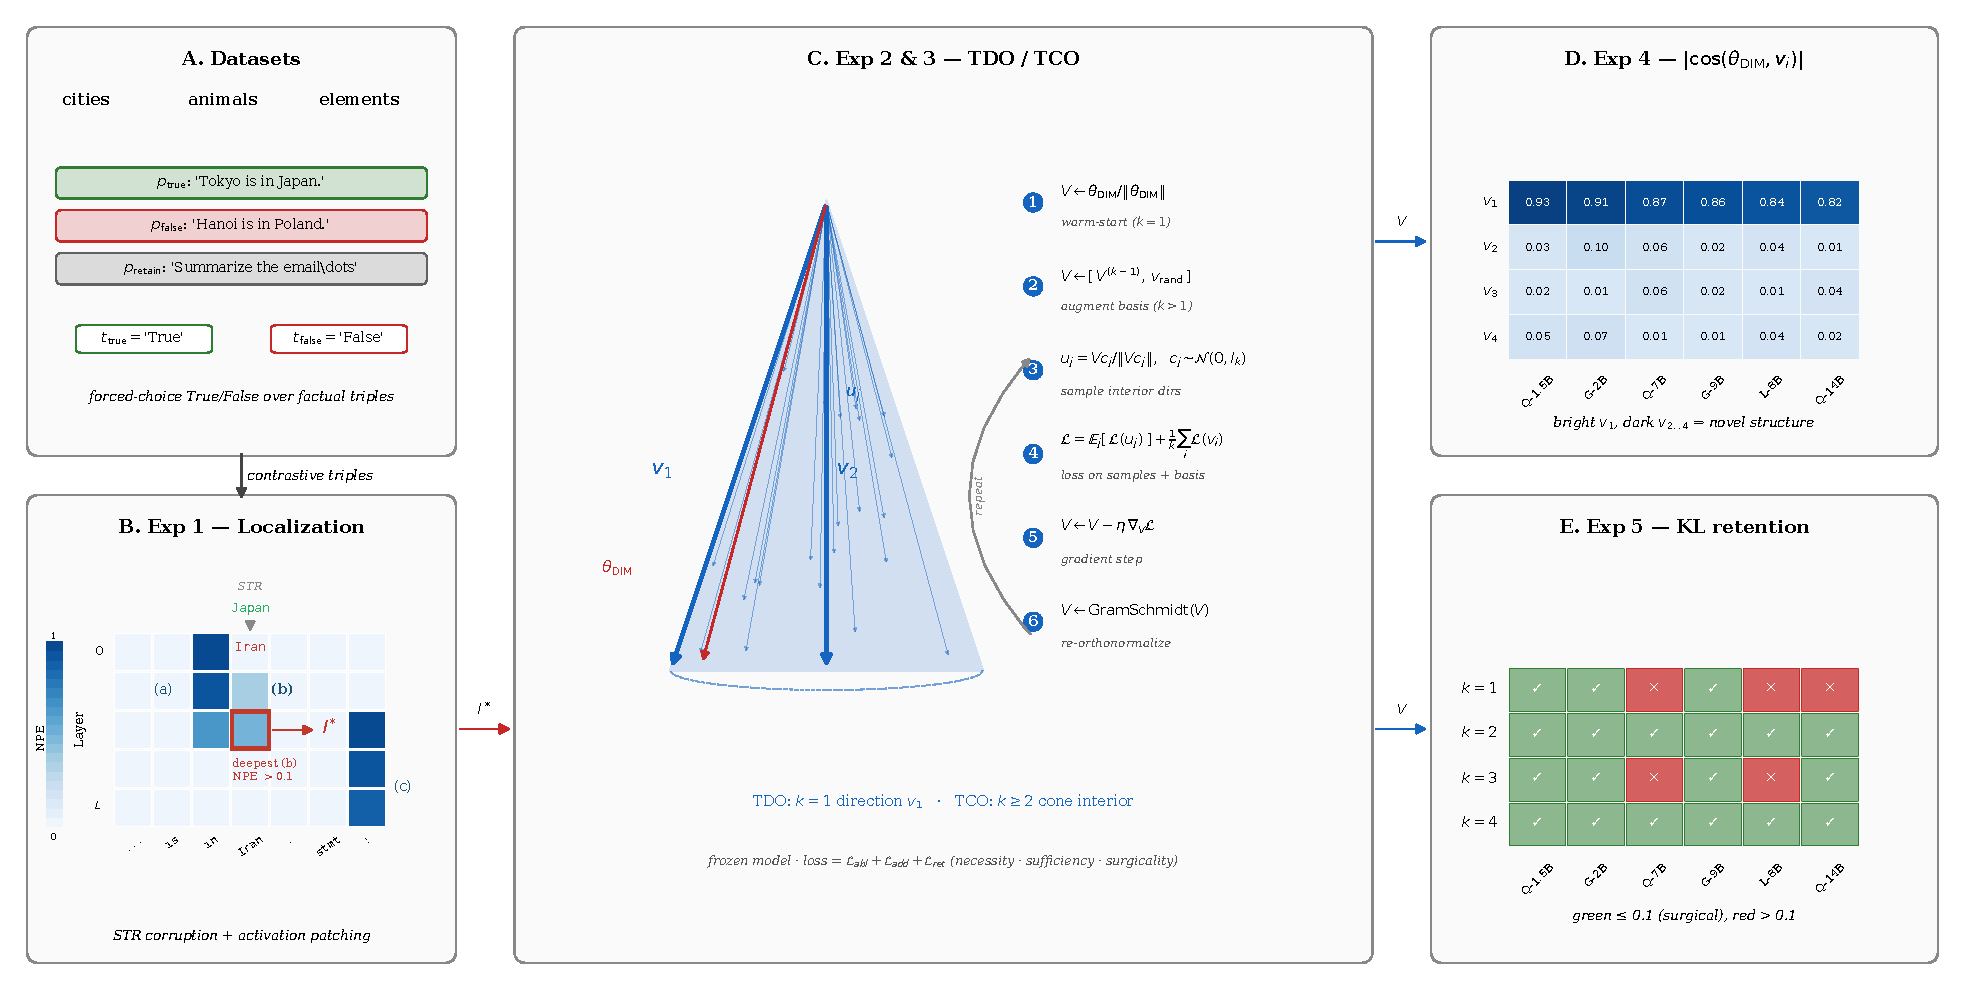
\includegraphics[width=\linewidth]{figures/fig_pipeline.pdf}

% \begin{tikzpicture}[
%     >={Stealth[length=2.2mm]},
%     box/.style   = {draw, rounded corners=2pt, inner sep=4pt, align=center},
%     panel/.style = {draw, rounded corners=3pt, inner sep=6pt, align=center,
%                     fill=gray!3, line width=0.6pt},
%     arr/.style   = {-{Stealth[length=2mm]}, line width=0.7pt},
%     label/.style = {font=\scriptsize\itshape}
% ]

% % ===========================================================================
% % PANEL A — DATASETS (left, ~22% width)
% % ===========================================================================
% \node[panel, minimum width=3.4cm, minimum height=4.6cm] (A) at (0,0) {};
% \node[anchor=north, font=\small\bfseries] at (A.north) {A. Datasets};

% % Three domain icons row
% \node[font=\scriptsize] at ($(A.north) + (-0.95,-0.55)$) {\bfseries cities};
% \node[font=\scriptsize] at ($(A.north) + ( 0.00,-0.55)$) {\bfseries animals};
% \node[font=\scriptsize] at ($(A.north) + ( 0.95,-0.55)$) {\bfseries elements};

% % Forced-choice triple, shown as colored bars (T/F/R)
% \node[box, fill=truecolor!18, draw=truecolor!60, minimum width=2.9cm,
%       minimum height=0.32cm, font=\tiny] (ptrue) at ($(A.center) + (0,0.4)$)
%       {$p_{\text{true}}$: ``Tokyo is in Japan.''};
% \node[box, fill=falsecolor!18, draw=falsecolor!60, minimum width=2.9cm,
%       minimum height=0.32cm, font=\tiny, below=1mm of ptrue] (pfalse)
%       {$p_{\text{false}}$: ``Hanoi is in Poland.''};
% \node[box, fill=retaincolor!15, draw=retaincolor!60, minimum width=2.9cm,
%       minimum height=0.32cm, font=\tiny, below=1mm of pfalse] (pretain)
%       {$p_{\text{retain}}$: ``Summarize the email\dots''};

% % Targets
% \node[box, draw=truecolor, minimum width=0.85cm, minimum height=0.32cm,
%       font=\tiny] (ttrue) at ($(pretain.south) + (-0.75,-0.45)$)
%       {$t_{\text{true}}{=}$``True''};
% \node[box, draw=falsecolor, minimum width=0.85cm, minimum height=0.32cm,
%       font=\tiny] (tfalse) at ($(pretain.south) + ( 0.75,-0.45)$)
%       {$t_{\text{false}}{=}$``False''};

% % Differentiator caption
% \node[font=\tiny\itshape, text width=3.2cm, align=center] at
%       ($(A.south) + (0,0.25)$) {forced-choice True/False over factual triples};

% % ===========================================================================
% % PANEL B — LOCALIZATION (top center-left, ~22% width)
% % ===========================================================================
% \node[panel, right=0.8cm of A, minimum width=3.4cm, minimum height=4.6cm,
%       yshift=1.3cm] (B) {};
% \node[anchor=north, font=\small\bfseries] at (B.north)
%      {B. Exp~1 — Localization};

% % Transformer column (schematic)
% \foreach \i/\y in {7/2.4, 6/2.0, 5/1.6, 4/1.2, 3/0.8, 2/0.4, 1/0.0} {
%   \draw[fill=methodcolor!15, draw=methodcolor!60, rounded corners=1pt]
%       ($(B.west) + (0.45, \y - 1.3)$) rectangle
%       ($(B.west) + (1.05, \y - 1.0)$);
% }
% % l* highlight (one of the middle blocks)
% \draw[fill=accentcolor!25, draw=accentcolor, line width=0.8pt, rounded corners=1pt]
%     ($(B.west) + (0.45, 0.4 - 1.3)$) rectangle
%     ($(B.west) + (1.05, 0.4 - 1.0)$);
% \node[font=\tiny, anchor=east, text=accentcolor]
%     at ($(B.west) + (0.42, 0.55 - 1.3)$) {$l^{*}$};

% % NPE mini-heatmap to the right of the column
% \foreach \i in {0,1,2,3,4} {
%   \foreach \j in {0,1,2,3,4,5,6} {
%     \pgfmathsetmacro{\val}{abs(sin((\i+\j)*20)) * 80}
%     \fill[methodcolor!\val] ($(B.west) + (1.35 + 0.18*\i, -1.3 + 0.21*\j)$)
%         rectangle ++(0.16,0.18);
%   }
% }
% % Group annotations
% \node[font=\tiny] at ($(B.west) + (2.5, -0.95)$) {(a)};
% \node[font=\tiny] at ($(B.west) + (2.5,  0.05)$) {(b)};
% \node[font=\tiny] at ($(B.west) + (2.5,  1.05)$) {(c)};

% \node[font=\tiny\itshape, text width=3.0cm, align=center]
%     at ($(B.south) + (0,0.25)$)
%     {STR corruption + denoising patch sweep};

% % Arrow from A to B
% \draw[arr] (A.east) -- node[above, label, pos=0.5]{contrastive triples}
%             (B.west |- A.east);
% % Arrow from B output to Panel C
% \draw[arr] (B.south) -- ++(0,-0.4)
%     node[right, label, pos=0.5]{\,\,$l^{*}$};

% % ===========================================================================
% % PANEL C — TCO with MC INTERIOR SAMPLING  (center, ~38% width — CENTERPIECE)
% % ===========================================================================
% \node[panel, right=0.8cm of B, minimum width=6.6cm, minimum height=6.0cm,
%       yshift=-0.65cm, fill=methodcolor!2] (C) {};
% \node[anchor=north, font=\small\bfseries] at (C.north)
%      {C. Exp~2 \& 3 — TDO / TCO with Monte-Carlo interior sampling};

% % Cone shape (translucent triangle as 2D sketch of a cone)
% \coordinate (apex) at ($(C.center) + (0,1.2)$);
% \coordinate (baseL) at ($(C.center) + (-1.6,-1.5)$);
% \coordinate (baseR) at ($(C.center) + ( 1.6,-1.5)$);
% \fill[conecolor] (apex) -- (baseL) -- (baseR) -- cycle;
% \draw[methodcolor, line width=0.6pt] (apex) -- (baseL);
% \draw[methodcolor, line width=0.6pt] (apex) -- (baseR);
% \draw[methodcolor!60, dashed, line width=0.4pt] (baseL) -- (baseR);

% % Cone elliptical base (perspective hint)
% \draw[methodcolor!60, dashed, line width=0.4pt]
%     (baseL) .. controls ($(C.center) + (-0.5,-1.7)$) and
%                        ($(C.center) + ( 0.5,-1.7)$) ..
%     (baseR);

% % Two basis vectors v1, v2 (bold arrows along cone edges)
% \draw[->, methodcolor, line width=1.1pt] (apex) -- (baseL)
%     node[pos=0.6, left=1pt, font=\scriptsize] {$v_1$};
% \draw[->, methodcolor, line width=1.1pt] (apex) --
%     ($(C.center) + (0.0,-1.5)$)
%     node[pos=0.7, left=1pt, font=\scriptsize] {$v_2$};

% % DIM vector (thin red, nearly aligned with v1, slightly off)
% \draw[->, accentcolor, line width=0.6pt] (apex) -- ($(baseL) + (0.25,0.05)$)
%     node[pos=0.55, right=1pt, font=\scriptsize\itshape] {$\theta_{\text{DIM}}$};

% % Interior MC samples (~25 thin gray arrows from apex into cone)
% \foreach \t in {-1.4,-1.2,-1.0,-0.8,-0.6,-0.4,-0.2,0,0.2,0.4,0.6,0.8,1.0,1.2,1.4} {
%   \pgfmathsetmacro{\dx}{\t * 1.0}
%   \pgfmathsetmacro{\dy}{-1.3 + 0.15*abs(\t)}
%   \draw[->, methodcolor!55, line width=0.25pt]
%       (apex) -- ($(apex) + (\dx, \dy)$);
% }
% \foreach \t in {-1.1,-0.7,-0.3,0.1,0.5,0.9,1.3} {
%   \pgfmathsetmacro{\dx}{\t * 0.65}
%   \pgfmathsetmacro{\dy}{-0.85 + 0.1*abs(\t)}
%   \draw[->, methodcolor!45, line width=0.25pt]
%       (apex) -- ($(apex) + (\dx, \dy)$);
% }

% % Callouts around the cone
% \node[font=\tiny, text=methodcolor, anchor=west]
%     at ($(C.east) + (-2.5,1.3)$)
%     {\itshape 256 samples / batch};
% \node[font=\tiny, text=methodcolor, anchor=west]
%     at ($(C.east) + (-2.5,1.0)$)
%     {\itshape (16 acc.\ steps $\times$ 16 dirs)};
% \node[font=\tiny, text=methodcolor, anchor=west]
%     at ($(C.east) + (-2.5,0.6)$)
%     {\itshape Gram--Schmidt every step};

% % Loss formula above cone
% \node[box, fill=white, draw=methodcolor!60, font=\tiny]
%     at ($(C.north) + (0,-0.55)$)
%     {$\mathcal{L} = \lambda_{\text{abl}}\mathcal{L}_{\text{abl}}
%                   + \lambda_{\text{add}}\mathcal{L}_{\text{add}}
%                   + \lambda_{\text{ret}}\mathcal{L}_{\text{ret}}$
%       \scriptsize applied to all 256 samples};

% % Warm-start chain (below cone)
% \node[font=\tiny, anchor=north] at ($(C.south) + (0,0.45)$)
%     {warm-start: $\theta_{\text{DIM}} \to V^{(1)} \to V^{(2)} \to V^{(3)} \to V^{(4)}$};
% \node[font=\tiny\itshape, anchor=north, text width=5.5cm, align=center]
%     at ($(C.south) + (0,0.25)$)
%     {(prev. basis $+$ random vector $+$ Gram--Schmidt)};

% % Frozen-model sidebar (right edge of C)
% \node[box, fill=gray!10, font=\tiny, text width=1.6cm, align=center, rotate=90]
%     at ($(C.east) + (-0.3,0)$)
%     {\textbf{Frozen LLM}\\[1pt]
%      Qwen-2.5 1.5/7/14B\\
%      Gemma-2 2/9B\\
%      Llama-3.1-8B};

% % ===========================================================================
% % PANEL D — ORTHOGONALITY (bottom left, Exp 4)
% % ===========================================================================
% \node[panel, below=0.7cm of A, minimum width=4.5cm, minimum height=2.3cm,
%       xshift=0.55cm] (D) {};
% \node[anchor=north, font=\small\bfseries] at (D.north)
%      {D. Exp~4 — $|\cos(\theta_{\text{DIM}}, v_i)|$};

% % Mini heatmap: 4 rows (i=1..4), 6 cols (models)
% \foreach \i [count=\r] in {1,2,3,4} {
%   \foreach \m [count=\c] in {qw15,gm2,qw7,gm9,ll8,qw14} {
%     \pgfmathsetmacro{\val}{ifthenelse(\i==1, 75 + 5*\c, 5 + 4*\c)}
%     \fill[methodcolor!\val] ($(D.center) + (-1.6 + 0.42*\c, 0.6 - 0.28*\r)$)
%         rectangle ++(0.4,0.26);
%   }
% }
% % v_i labels
% \foreach \i [count=\r] in {$v_1$,$v_2$,$v_3$,$v_4$} {
%   \node[font=\tiny, anchor=east]
%       at ($(D.center) + (-1.45, 0.73 - 0.28*\r)$) {\i};
% }
% \node[font=\tiny\itshape, anchor=north]
%     at ($(D.south) + (0,0.25)$) {bright $v_1$, dark $v_{2..4}$ $\Rightarrow$ novel structure};

% % ===========================================================================
% % PANEL E — KL RETENTION (bottom right, Exp 5)
% % ===========================================================================
% \node[panel, below=0.7cm of C, minimum width=4.5cm, minimum height=2.3cm,
%       xshift=-0.55cm] (E) {};
% \node[anchor=north, font=\small\bfseries] at (E.north)
%      {E. Exp~5 — KL retention};

% % Heatmap: 4 rows (k=1..4), 6 cols (models); green if ≤ 0.1, red otherwise
% % Hand-coded based on actual Exp 5 numbers
% \def\kldata{
%   % k=1 row (top): qw15 ✓, gm2 ✓, qw7 ✗, gm9 ✓, ll8 ✗, qw14 ✗
%   1/1/g, 1/2/g, 1/3/r, 1/4/g, 1/5/r, 1/6/r,
%   % k=2 row (all surgical)
%   2/1/g, 2/2/g, 2/3/g, 2/4/g, 2/5/g, 2/6/g,
%   % k=3 row: qw7 ✗, ll8 ✗
%   3/1/g, 3/2/g, 3/3/r, 3/4/g, 3/5/r, 3/6/g,
%   % k=4 row (all surgical)
%   4/1/g, 4/2/g, 4/3/g, 4/4/g, 4/5/g, 4/6/g
% }
% \foreach \r/\c/\col in \kldata {
%   \ifnum\pdfstrcmp{\col}{g}=0
%     \fill[truecolor!55] ($(E.center) + (-1.6 + 0.42*\c, 0.6 - 0.28*\r)$)
%        rectangle ++(0.4,0.26);
%   \else
%     \fill[falsecolor!75] ($(E.center) + (-1.6 + 0.42*\c, 0.6 - 0.28*\r)$)
%        rectangle ++(0.4,0.26);
%   \fi
% }
% % k labels
% \foreach \i [count=\r] in {$k{=}1$,$k{=}2$,$k{=}3$,$k{=}4$} {
%   \node[font=\tiny, anchor=east]
%       at ($(E.center) + (-1.45, 0.73 - 0.28*\r)$) {\i};
% }
% \node[font=\tiny\itshape, anchor=north]
%     at ($(E.south) + (0,0.25)$)
%     {green $\le 0.1$ (surgical), red $> 0.1$};

% % ===========================================================================
% % Connectors C -> D, C -> E
% % ===========================================================================
% \draw[arr] (C.south west) .. controls +(-0.5,-0.6) and +(0.3,0.5) .. (D.north east)
%     node[label, pos=0.45, above] {$V$};
% \draw[arr] (C.south east) .. controls +( 0.5,-0.6) and +(-0.3,0.5) .. (E.north west)
%     node[label, pos=0.45, above] {$V$};

% \end{tikzpicture}

\caption{
\textbf{Pipeline overview.} Contrastive factual triples ($p_{\text{true}}$,
$p_{\text{false}}$, $p_{\text{retain}}$) over three domains (cities, animals,
elements) drive a frozen instruction-tuned LLM.
\textbf{(A)} Forced-choice True/False format with a retain set of filtered
Alpaca instructions.
\textbf{(B)} Exp~1 localizes the truth-mediating hidden state $l^{*}$ via
symmetric-token-replacement corruption + denoising activation patching, with
three causally implicated groups (a)(b)(c).
\textbf{(C)} Exp~2 / Exp~3 optimize a $k$-dimensional orthonormal cone basis
$V$ at $l^{*}$. At every accumulation step, $16$ directions are
Monte-Carlo--sampled from the cone interior, the composite loss
$\mathcal{L} = \lambda_{\text{abl}}\mathcal{L}_{\text{abl}} +
\lambda_{\text{add}}\mathcal{L}_{\text{add}} +
\lambda_{\text{ret}}\mathcal{L}_{\text{ret}}$ is applied to all of them, and
modified Gram--Schmidt re-orthogonalizes $V$ after each step; effective
$256$ samples per batch force the cone \emph{interior} to mediate truth.
\textbf{(D)}~Exp~4 verifies $|\cos(\theta_{\text{DIM}}, v_i)| \approx 0$ for
$i \ge 2$.
\textbf{(E)}~Exp~5 verifies surgicality with mean KL on a $100$-prompt
retain set (threshold $0.1$).
}
\label{fig:pipeline}
\end{figure*}

I study factual knowledge as a forced binary choice: the model is shown a
factual statement and must decide whether it is ``True'' or ``False''. Given a
frozen instruction-tuned model $f$, my goal is to find a subspace of $f$'s
residual stream that causally controls this decision, a set of directions
whose manipulation flips the model's verdict.

\Cref{sec:axioms} states the two causal properties a candidate truth direction
must satisfy; \Cref{sec:loc} describes the activation-patching step that selects
a target layer $l^{*}$ per model; \Cref{sec:dim} gives the DIM baseline and the
magnitude calibration $\alpha = \|\dimv\|_2$; \Cref{sec:tdo} introduces TDO;
\Cref{sec:tco} extends it to the $k$-dimensional cone; and \Cref{sec:eval}
defines the evaluation protocols.

\subsubsection*{Factual evaluation.}
Concretely, following \citet{marksGeometryTruthEmergent2024}, each prompt uses a
few-shot, in-context format rather than a conversational one:

\begin{quote}\ttfamily\small The city of Tokyo is in Japan. This statement is:
True\\
The city of Hanoi is in Poland. This statement is: False\\
The city of Chicago is in Canada. This statement is:
\end{quote}
%
\noindent The model's next-token distribution is restricted to the two token IDs
$t_{\text{true}}=$\,``True'' and $t_{\text{false}}=$\,``False''. The fixed
suffix ``\,This statement is:\,'' separates the adverbial phrase and the closing
punctuation, which together carry the truth-relevant edit, from the position at
which the final layer reads out the prediction; this separation lets the
activation-patching step (\Cref{sec:loc}) isolate the truth signal before
readout. The few-shot format also reduces interference from
instruction-following circuits introduced during RLHF.

The training data are triples $(p_{\text{true}}, p_{\text{false}},
p_{\text{retain}})$: two factual statements with opposite truth value and one
filtered Alpaca instruction with no factual-recall keywords.


\subsection{Truth mediation properties}
\label{sec:axioms}

Let $f$ be a frozen autoregressive transformer with $L \in \mathbb{N}$ layers
and hidden size $d \in \mathbb{N}$, and let $x^{(l)}_{i}(p) \in \mathbb{R}^{d}$
denote its residual-stream activation at layer $l$ and token position $i$ on
prompt $p$. A candidate truth direction is a unit vector $r \in \mathbb{S}^{d-1}
= \{v \in \mathbb{R}^{d} : \|v\|_2 = 1\}$; its multi-dimensional generalization
is a vector $r \in \mathrm{Cone}(V)$ drawn from the concept cone
$\mathrm{Cone}(V) = \{\sum_{i=1}^{k} \lambda_i v_i : \lambda_i \ge 0\} \setminus
\{0\}$ spanned by an orthonormal basis $V = [v_1, \ldots, v_k] \in \mathbb{R}^{d
\times k}$, of which the single-direction case is $k=1$. Its causal role is
probed by intervening on the activations $\{x^{(l)}_{i}(p)\}_{l,i}$ through the
two operations below, and $r$, or, more generally, a concept cone
$\mathrm{Cone}(V) \subseteq \mathbb{R}^{d}$ of such directions, is admissible
only if these interventions certify the two causal axioms of \Cref{def:axioms}.


\subsubsection*{Intervention operations.}
\emph{Directional ablation} $\fablate[r]$ projects the stream onto the subspace
orthogonal to $r$ at every layer and position:
%
\begin{equation}
\forall\, i\;\forall\, l\quad
\tilde{x}^{(l)}_i = x^{(l)}_i
  - \hat{r}\,\hat{r}^{\!\top} x^{(l)}_i,
\end{equation}
%
where $\hat{r}$ is the unit vector along $r$. If the verdict flips from ``True''
to ``False'' after ablation, $r$ was causally necessary.\\
\emph{Activation addition} $\fadd[r,l^{*}](p_{\text{false}})$ injects a scaled
truth signal at a single layer $l^{*}$:
%
\begin{equation}
\forall\, i\quad
\tilde{x}^{(l^{*})}_i = x^{(l^{*})}_i + \alpha \cdot r.
\end{equation}
%
If a false statement flips to ``True'' under addition, $r$ was causally
sufficient to override the original judgment. Following
\citet{arditiRefusalLanguageModels2024}, ablation is applied across all layers
and token positions, and addition at the single selected layer $l^*$
(\Cref{sec:loc}).

\begin{definition}[Truth mediation]
\label{def:axioms}
A direction $r \in \mathbb{R}^{d}$ at layer $l^{*}$ \emph{mediates truth} if:
\begin{enumerate}
\item \textbf{Monotonic scaling.} For every false statement $p_{\text{false}}$,
the probability of ``True'' under $\fadd[r,l^{*}](p_{\text{false}})$ increases
monotonically with the coefficient $\alpha \in [0, \alpha_{\max}]$.
\item \textbf{Surgical factuality ablation.} The directional ablation
$\fablate[r](p_{\text{true}})$ satisfies (i) \emph{causal necessity}: on true statements
$p_{\text{true}}$, the model flips its judgment from ``True'' to ``False'' with
high probability; and (ii) \emph{functional specificity}: on retain prompts
$p_{\text{retain}}$, the output distribution is preserved ($\mathrm{KL} < 0.1$
per \cite{arditiRefusalLanguageModels2024}).
\end{enumerate}
A $k$-dim cone basis $V$ mediates truth if every direction sampled from the
relative cone $\mathrm{Cone}(V)$ satisfies both axioms.
\end{definition}

The cone version of \Cref{def:axioms} motivates the Monte-Carlo sampling in
\Cref{sec:tco}: optimizing only on the basis vectors leaves the interior of
$\mathrm{Cone}(V)$ unconstrained, so it need not satisfy the $k$-dim version of
the axioms.

Two metrics quantify these axioms and are reported throughout. The
\textbf{Answer Switching Rate} (ASR) is the fraction of factual prompts whose
argmax token flips under intervention: $\mathrm{ASR}_{\text{abl}}$ ablates
$p_{\text{true}}$ and counts flips to ``False'' (necessity);
$\mathrm{ASR}_{\text{add}}$ adds to $p_{\text{false}}$ and counts flips to
``True'' (sufficiency). \textbf{KL retention} $\mathrm{KL}(p_{r} \| p_{0})$ is
the divergence between the last-$30$-token distributions on $p_{\text{retain}}$
with and without ablation of $r$ (functional specificity).

\subsection{Localizing the truth-mediating layer}
\label{sec:loc}

Both TDO and TCO optimize at a single layer $l^{*}$, and running the full
optimization at every layer is too expensive, so I first localize, per model,
the layer whose residual-stream states most strongly mediate the truth judgment.

To do this I use denoising activation
patching~\citep{heimersheimHowUseInterpret2024}, following
\citet{marksGeometryTruthEmergent2024}. For each model I sample $50$ contrastive
pairs per dataset (cities, animals, elements). Each clean prompt
$p_{\text{clean}}$ is corrupted to $p_{\text{corrupt}}$ by Symmetric Token
Replacement (STR): the object token is swapped for a semantically related
alternative that flips the ground-truth label while preserving syntactic
structure and token count. I then cache the clean-run activations, re-run the
model on $p_{\text{corrupt}}$, and restore a single activation at position $i$,
layer $l$ from the clean cache. To measure how much a layer contributes, I use
the \textbf{logit difference} $M(p) = \mathrm{logit}(p)_{t_{\text{true}}} -
\mathrm{logit}(p)_{t_{\text{false}}}$; following
\citet{zhangBESTPRACTICESACTIVATION2024} I prefer it to a probability-based
metric, since probability can miss components that contribute negatively to the
correct answer, while the logit difference is linear in the final residual
stream and so decomposes cleanly under patching.
Writing $M_{\text{clean}}$, $M_{\text{corrupt}}$, and $M_{\text{patched}}$ for
the logit difference on the clean run, the corrupted run, and the restored run,
the effect of that restoration is the normalized patching effect
%
\begin{equation}
\mathrm{NPE}(l, i) =
\frac{M_{\text{patched}} - M_{\text{corrupt}}}
     {M_{\text{clean}} - M_{\text{corrupt}}},
\end{equation}
%
which lies in $[0, 1]$: it is $1$ when restoring $(l, i)$ fully recovers clean
performance and $0$ at the corrupted baseline.

Sweeping $\mathrm{NPE}$ over every layer and position, then aggregating across
models and datasets, reveals three groups of causally implicated hidden states,
matching \citet{marksGeometryTruthEmergent2024}: group~(a), the entity token
that STR perturbs, encoding the factual association; group~(b), the
end-of-statement punctuation in mid layers, where clause-level information is
aggregated into a propositional judgment; and group~(c), the colon token ``\,:''
in mid-to-late layers, which encodes the model's prediction (applying the
decoder head to these states gives top logits for ``True''/``False''). I take
$l^{*}$ from group~(b), the propositional judgment itself rather than its
readout in (c), as the most-downstream layer there with mean $\mathrm{NPE} >
0.1$. Across all six models the selected layer falls at normalized depth
$0.44$--$0.69$ (\Cref{tab:master}).

\begin{figure}[t]
\centering
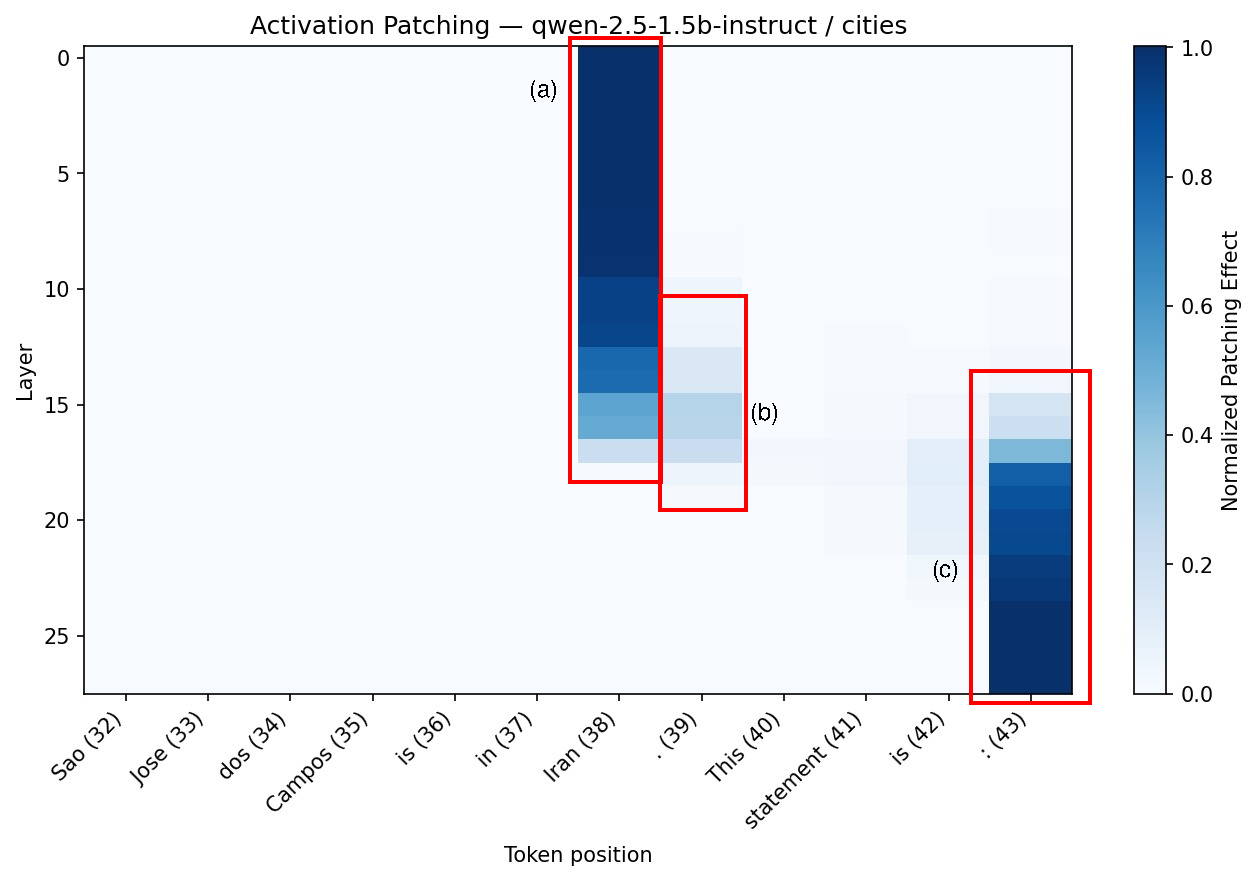
\includegraphics[width=0.8\columnwidth]{figures/qwen-2.5-1.5b-instruct_cities_heatmap.pdf}
\caption{Activation patching heatmap for Qwen-2.5-1.5B-Instruct on the cities
domain, averaged over all $50$ statement pairs.}
\label{fig:patching_qwen1.5b}
\end{figure}

This reduces the search space for all later optimization to a single $(l^{*},
-5)$ pair per model.\footnote{The position $i = -5$ follows from the prompt
structure: for all six tokenizers the four trailing tokens after the final word
of the factual statement are the fixed suffix ``\,This statement is:\,'', so
position $-5$ lands on the end-of-statement punctuation.} DIM, TDO, and TCO then
all operate at the layer most causally implicated for that model, so the
cross-family comparison does not rely on a fixed depth.

\subsection{DIM baseline and magnitude calibration}
\label{sec:dim}
A linear baseline both anchors the comparison and gives a starting point for
optimization. Following \cite{marksGeometryTruthEmergent2024,
arditiRefusalLanguageModels2024} I compute $\dimv = \bmu_{+} - \bmu_{-}$, where
$\bmu_{+}$ and $\bmu_{-}$ are the mean activations at $(l^{*}, -5)$ over the
true and false training subsets. $\dimv$ is normalized to a unit vector for
ablation and used at its natural norm $\alpha := \|\dimv\|_{2}$ for addition.
Calibrating $\alpha$ to the model's own representational scale at $l^{*}$,
rather than tuning it by hand, removes one degree of freedom; per-model $\alpha$
ranges from $4.07$ (Llama-3.1-8B) to $106.56$ (Gemma-2-9B), reflecting large
differences in residual-stream norm across families (\Cref{tab:master}).

\subsection{Truth Direction Optimization (TDO)}
\label{sec:tdo}

DIM finds a direction that maximally separates the means of true and false
activations, but mean separation does not guarantee causal mediation: a
separating vector may fail to flip the model under ablation and may not
preserve general capabilities. I therefore encode the causal axioms
(\Cref{def:axioms}) directly into loss functions and recover a corresponding
truth direction $r \in \mathbb{R}^{d}$ by gradient descent.

For the sufficiency property, I train the model to predict ``True'' on false
statements $p_{\text{false}}$ by running $f$ with a modified forward pass
$\fadd[r,l^{*}](p_{\text{false}})$ that adds $r$ to the activations at layer
$l^{*}$ with scaling coefficient $\alpha$, minimizing the cross-entropy between
the model output and the target token $t_{\text{true}}$. For the necessity
property, I symmetrically compute the cross-entropy between the target token
$t_{\text{false}}$ and the output of a modified forward pass
$\fablate[r]$ that projects $r$ out of every residual stream position,
driving the model to predict ``False'' on true statements $p_{\text{true}}$.
A key strength of the gradient-based approach is the ability to control any
predefined objective, which lets me bound the extent to which unrelated
computations are perturbed. For this, I use a retain loss based on the
Kullback--Leibler (KL) divergence to ensure that directional ablation of $r$
on retain prompts $p_{\text{retain}}$ does not shift the model's output
distribution. The three terms combine into a composite loss
\[
\mathcal{L}(r) =
   \lambda_{\text{abl}} \Labl(r)
 + \lambda_{\text{add}} \Ladd(r)
 + \lambda_{\text{ret}} \Lret(r),
\]
where
\begin{align*}
\Labl(r) &= \mathrm{CE}\!\left(f_{\text{ablate}(r)}(p_{\text{true}}),\;
                                t_{\text{false}}\right)
  &\text{(necessity)},\\
\Ladd(r) &= \mathrm{CE}\!\left(f_{\text{add}(r,l^{*},\alpha)}(p_{\text{false}}),\;
                                t_{\text{true}}\right)
  &\text{(sufficiency)},\\
\Lret(r) &= \mathrm{KL}\!\left(f_{\text{ablate}(r)}(p_{\text{retain}})\;\|\;
                                f(p_{\text{retain}})\right)
  &\text{(surgicality)}.
\end{align*}
I initialize $r$ from $\dimv / \|\dimv\|$ (warm start), placing the optimizer
in the discriminative region rather than at a random point on the unit sphere.
The loss weights $(\lambda_{\text{abl}}, \lambda_{\text{add}},
\lambda_{\text{ret}}) = (1.0, 0.2, 1.0)$ are taken from
\citet[Tab.~3]{wollschlagerGeometryRefusalLarge2025} and held fixed across all
six models (\Cref{tab:hyperparams}). \Cref{alg:tdo} gives the full procedure.

\begin{algorithm}[t]
\caption{Truth Direction Optimization (TDO)}
\label{alg:tdo}
\begin{algorithmic}[1]
\Require Frozen model $f$, scaling coefficient $\alpha$, addition layer $l^{*}$,
  learning rate $\eta$, loss weights $\lambda_{\text{abl}},
  \lambda_{\text{add}}, \lambda_{\text{ret}}$, and data $\mathcal{D} =
  \{(p_{\text{true},i},\; p_{\text{false},i},\;
  p_{\text{retain},i})\}_{i=1}^{N}$.
\Ensure Truth direction $r$
\State $r \leftarrow \theta_{\text{DIM}} / \|\theta_{\text{DIM}}\|_2$
  \Comment{warm-start from DIM}
\While{not converged}
  \State Sample batch $\mathbf{B} \sim \mathcal{D}$
  \State $\mathcal{L} \leftarrow \textsc{ComputeLoss}(r, f, \mathbf{B})$
  \State $r \leftarrow r - \eta\, \nabla_{r} \mathcal{L}$
  \State $r \leftarrow r / \|r\|_2$
    \Comment{renormalize to unit sphere}
\EndWhile \\
\Function{ComputeLoss}{$r, f, \mathbf{B}$}
  \State $p_{\text{true}},\, p_{\text{false}},\, p_{\text{retain}} \leftarrow
    \mathbf{B}$
  \State $\mathcal{L}_{\text{abl}} \leftarrow
    \mathrm{CE}\,\bigl(f_{\text{ablate}(r)}(p_{\text{true}}),\;
    t_{\text{false}}\bigr)$
  \State $\mathcal{L}_{\text{add}} \leftarrow
    \mathrm{CE}\,\bigl(f_{\text{add}(r,\,l^{*},\,\alpha)}(p_{\text{false}}),\;
    t_{\text{true}}\bigr)$
  \State $\mathcal{L}_{\text{ret}} \leftarrow
    \mathrm{KL}\,\bigl(f_{\text{ablate}(r)}(p_{\text{retain}})\;\|\;
    f(p_{\text{retain}})\bigr)$
  \State \Return $\lambda_{\text{abl}}\,\mathcal{L}_{\text{abl}} +
    \lambda_{\text{add}}\,\mathcal{L}_{\text{add}} +
    \lambda_{\text{ret}}\,\mathcal{L}_{\text{ret}}$
\EndFunction
\end{algorithmic}
\end{algorithm}


\subsection{Truth Cone Optimization (TCO)}
\label{sec:tco}

\Cref{tab:tdo_vs_dim} shows that even TDO at $k = 1$ fails for the three larger
models on ablation (e.g.\ Qwen-2.5-7B: $\mathrm{ASR} = 0.020$). If truth
occupies a multi-dimensional linear subspace, one direction can only capture a
projection of it. I therefore extend TDO to higher dimensions by searching for
regions in activation space where all vectors mediate the truth verdict. For
this, I optimize an orthonormal basis $V = [v_1, \ldots, v_k] \in \mathbb{R}^{d
\times k}$ spanning a $k$-dimensional polyhedral cone $\mathrm{Cone}(V) =
\{\sum_{i=1}^{k} \lambda_i v_i \mid \lambda_i \ge 0\} \setminus \{0\}$, where
every direction $r \in \mathrm{Cone}(V)$ satisfies the causal axioms
(\Cref{def:axioms}). The constraint $\lambda_i \ge 0$ ensures that directions
within the cone consistently strengthen the truth signal; allowing negative
coefficients could introduce opposing effects and reduce overall effectiveness.
Orthogonality of the basis vectors prevents the optimizer from collapsing onto
co-linear directions. In practice, activation-space directions cannot be scaled
arbitrarily without model degeneration, which effectively bounds $\lambda_i$.

A naive extension of TDO would optimize only the basis vectors, but this causes
\emph{basis collapse}: the loss is satisfied at each $v_i$ while interior
directions of the cone remain unconstrained. I avoid this by evaluating the
composite loss both on the basis vectors and on Monte-Carlo samples drawn from
the cone interior at every step. Computing the loss on the basis vectors
improves stability and tightens the lower bound of the ASR, since the basis
vectors form the cone boundary and tend to degrade first. After each gradient
step, I re-project the basis onto the cone via modified Gram--Schmidt
orthonormalization, which restores orthonormality of $V$.

Sampling the interior requires care. Directional ablation depends only on the
normalized $\hat{r}$, so what matters is the \emph{direction} of the sample,
not its magnitude. A natural choice would be to draw non-negative coefficients
$\lambda_i$, form a convex combination $r = \sum_i \lambda_i v_i$, and
normalize; but the map from coefficients to normalized directions is uneven,
and most such samples cluster near the basis vectors after normalization,
biasing the estimate toward the cone boundary. I instead sample directions
uniformly from the non-negative orthant of the unit sphere in the cone's
coordinate space, exploiting the rotational symmetry of the isotropic
Gaussian: at each step, $16$ directions $\{u_j\}$ are drawn by sampling
$c_j \sim \mathcal{N}(0, I_k)$, taking component-wise absolute values to fold
the mass into the positive orthant, and setting
$u_j = |c_j| / \| |c_j| \|_2$. Each $u_j \in \mathbb{R}^k$ is a unit vector of
non-negative coefficients expressed in the basis of the cone; the map
$r = V u_j$ realizes it as a direction in the model's residual stream
$\mathbb{R}^d$, where the intervention is applied. This Gaussian-based scheme
yields uniform coverage of the cone and avoids the boundary bias of
convex-combination sampling~\citep{wollschlagerGeometryRefusalLarge2025}.

Initialization is incremental: for $k = 1$, I set $V$ from $\dimv$ as in TDO;
for $k > 1$, I augment the previous $(k{-}1)$-cone basis with one random unit
vector and re-orthonormalize, adding a single degree of freedom per increment.
All other hyperparameters are inherited from TDO (\Cref{tab:hyperparams}).
\Cref{alg:tco} gives the full procedure.

\begin{algorithm}[t]
\caption{Truth Cone Optimization (TCO)}
\label{alg:tco}
\begin{algorithmic}[1]
\Require Frozen model $f$, scaling coefficient $\alpha$, addition layer $l^{*}$,
  learning rate $\eta$, loss weights $\lambda_{\text{abl}},
  \lambda_{\text{add}}, \lambda_{\text{ret}}$, cone dimension $k$, and data
  $\mathcal{D} = \{(p_{\text{true},i},\; p_{\text{false},i},\;
  p_{\text{retain},i})\}_{i=1}^{N}$.
\Ensure Orthonormal cone basis $V = [v_1, \ldots, v_k]$
\If{$k = 1$}
  \State $V \leftarrow \theta_{\text{DIM}} / \|\theta_{\text{DIM}}\|_2$
\Else
  \State $V \leftarrow [V^{(k-1)},\; v_{\text{rand}}]$
    \Comment{augment previous basis}
  \State $V \leftarrow \textsc{GramSchmidt}(V)$
\EndIf
\While{not converged}
  \State Sample batch $\mathbf{B} \sim \mathcal{D}$
  \State $\mathcal{L}_{\text{sample}} \leftarrow
    \mathbb{E}_{u \sim \textsc{Sample}(V)}
    \bigl[\textsc{ComputeLoss}\,(u,\, f,\, \mathbf{B})\bigr]$
  \State $\mathcal{L}_{\text{basis}} \leftarrow \frac{1}{k} \sum_{i=1}^{k}
    \textsc{ComputeLoss}\,(v_i,\, f,\, \mathbf{B})$
  \State $\mathcal{L} \leftarrow \mathcal{L}_{\text{sample}} +
    \mathcal{L}_{\text{basis}}$
  \State $V \leftarrow V - \eta\, \nabla_{V} \mathcal{L}$
  \State $V \leftarrow \textsc{GramSchmidt}(V)$
    \Comment{re-orthonormalize}
\EndWhile \\
\Function{Sample}{$V$}
  \State $s \sim \text{Unif}(x \in \mathbb{R}^k_+ : \|x\|_2 = 1)$
  \State $r = V s$
  \State \Return $r$
\EndFunction
\end{algorithmic}
\end{algorithm}


\subsection{Evaluation protocol}
\label{sec:eval}

Two evaluations check whether a learned cone captures \emph{novel} structure and
whether it does so without damaging general capabilities.

\subsubsection*{Geometric alignment with DIM.}
A high-ASR cone that merely replicates the DIM direction $k$ times would be
trivial. For each cone of dimension $k \in \{1, 2, 3, 4\}$ I compute the cosine
alignment $|\cos(\dimv, v_i)|$ for every basis vector and a cone adds novel
structure if $|\cos(\dimv, v_i)| \approx 0$ for multiple $v_i$ while each
direction stays individually causally effective (\Cref{tab:orthogonality}).

\subsubsection*{KL retention on filtered Alpaca.}
High ASR result is useless if the intervention destroys general capabilities.
For each (model,~$k$) pair I sample $32$ directions from the cone interior
(\Cref{alg:tco}) and compute the mean KL divergence between the ablated and
clean model over the last $30$ token positions of $100$ held-out Alpaca
instructions filtered of factual-recall keywords. A cone is \emph{surgical} if
the mean MC~KL falls below $0.1$~\citep{arditiRefusalLanguageModels2024}, about
$96{,}000$ token-level comparisons per cone.

\section{Experiments}
\label{sec:exp}

% ============================================================================
%  Required packages: booktabs, xcolor, colortbl, multirow, siunitx (optional)
%
%  Color macros (define once in main preamble):
%      \definecolor{bestcolor}{HTML}{C62828}    % deep red for best
%      \definecolor{secondcolor}{HTML}{1565C0}  % deep blue for second-best
%      \definecolor{failcolor}{HTML}{FFCDD2}    % light red row tint for KL>0.1
%      \definecolor{passcolor}{HTML}{C8E6C9}    % light green row tint for KL<0.1
%      \newcommand{\best}[1]{\textcolor{bestcolor}{\textbf{#1}}}
%      \newcommand{\second}[1]{\textcolor{secondcolor}{\underline{#1}}}
% ============================================================================

% ----------------------------------------------------------------------------
% TABLE 1 — Master single-row-per-model summary (the decisive table).
% Place at the opening of §4 Experiments.
% ----------------------------------------------------------------------------
\begin{table*}[!ht]
\centering
\caption{%
\textbf{Cross-model summary.}
$l^{*}$: target hidden-state layer from Exp~1. $\alpha = \|\theta_{\text{DIM}}\|_{2}$:
intervention magnitude. ASR$_{\text{abl}}$: in-distribution Answer Switching Rate
under ablation. ``Surgical'' columns mark whether $\mathrm{mean\,KL} < 0.1$ on the
retain set. Higher ASR ($\uparrow$) and lower KL ($\downarrow$) are better.
The three models that fail \emph{both} axes at $k=1$ (\colorbox{failcolor!60}{red row tint})
all recover \emph{both} at $k=2$.}
\label{tab:master}
\small
\resizebox{\columnwidth}{!}{
\begin{tabular}{lrrrrrrcc}
\toprule
Model & $l^{*}$ & $\alpha$
      & \multicolumn{1}{c}{DIM ASR$_{\text{abl}}\!\uparrow$}
      & \multicolumn{1}{c}{TDO ASR$_{\text{abl}}\!\uparrow$}
      & \multicolumn{1}{c}{$k{=}2$ ASR$\!\uparrow$}
      & \multicolumn{1}{c}{$k{=}2$ KL$\!\downarrow$}
      & Surg.\ $k{=}1$ & Surg.\ $k{=}2$ \\
\midrule
Qwen-2.5-1.5B-Instruct & 17 &  13.05 & 0.010 & \best{1.000} & 1.000 & 0.008 & \checkmark & \checkmark \\
Gemma-2-2B-it          & 15 &  84.52 & 0.216 & \best{1.000} & 1.000 & 0.004 & \checkmark & \checkmark \\
\rowcolor{failcolor!50}
Qwen-2.5-7B-Instruct   & 18 &  26.61 & 0.000 & 0.020        & \best{1.000} & 0.037 & $\times$ & \checkmark \\
Gemma-2-9B-it          & 24 & 106.56 & 0.000 & 0.774        & \best{1.000} & 0.001 & \checkmark & \checkmark \\
\rowcolor{failcolor!50}
Llama-3.1-8B-Instruct  & 14 &   4.07 & 0.020 & \best{1.000} & 1.000 & 0.017 & $\times$ & \checkmark \\
\rowcolor{failcolor!50}
Qwen-2.5-14B-Instruct  & 30 &  48.25 & 0.000 & 0.658        & \best{1.000} & 0.009 & $\times$ & \checkmark \\
\bottomrule
\end{tabular}
}
\end{table*}



\subsection{Experimental setup}
\label{sec:setup}
\subsubsection*{Models.}
Six instruction-tuned models from three families: Qwen-2.5 (1.5B, 7B,
14B)~\cite{yang2024qwen25}, Gemma-2 (2B, 9B)~\cite{gemmateam2024gemma2}, and
Llama-3.1-8B~\cite{grattafiori2024llama3}. All are loaded via
nnsight~\cite{fiotto-kaufmanNNsightNDIFDemocratizing2025} on a RunPod NVIDIA A40
48GB instance.
\subsubsection*{Datasets.}
Three True/False datasets: \textbf{cities} (``The city of [City]
is in [Country]'', $1\,496$ statements)~\cite{marksGeometryTruthEmergent2024},
\textbf{animals} (``A [Animal] is a mammal'', $504$), \textbf{elements} (``The
symbol for [Element] is [Symbol]'', $930$), plus a \textbf{retain} set of $100$
filtered Alpaca instructions. Each factual dataset is split $80$/$20$ for ID
evaluation; OOD evaluation trains on cities and animals and evaluates on
elements.
\subsubsection*{Metrics.}
$\mathrm{ASR}_{\text{abl}}$, $\mathrm{ASR}_{\text{add}}$, and KL retention
(\Cref{sec:axioms}); logit difference for localization (\Cref{sec:loc}).
Hyperparameters in \Cref{tab:hyperparams}.



\subsection{TDO improves on the DIM baseline (RQ1)}
\label{sec:exp_tdo}

\textbf{Research question:} Does gradient-based 1-D optimization recover
causally more precise directions than the Difference-in-Means baseline at
matched layer and intervention magnitude?

\Cref{tab:tdo_vs_dim} reports $\mathrm{ASR}_{\text{abl}}$ and
$\mathrm{ASR}_{\text{add}}$ for both methods, ID and OOD.

\begin{itemize}[leftmargin=*,nosep]
\item \textbf{TDO closes the DIM ablation gap on five of six models.} For
Qwen-2.5-1.5B, Gemma-2-2B, Gemma-2-9B, Llama-3.1-8B, and Qwen-2.5-14B, TDO
ablation ASR moves from $\le 0.216$ (DIM) to between $0.658$ and $1.000$. The
composite loss optimizes $\Labl$ directly, while DIM optimizes only mean
separation. The OOD numbers suggest TDO is not memorizing entity-specific noise:
TDO ablation OOD stays $\ge 0.125$ on every model except Qwen-2.5-7B.

\item \textbf{TDO at $k=1$ fails for Qwen-2.5-7B.} Here both DIM and TDO give
near-zero ablation ASR ($0.000$ and $0.020$). This is a clear failure of the
$1$-D method on one model and motivates \Cref{sec:exp_cone}, where $k=2$ reaches
ASR $= 1.000$ ID for it.
\end{itemize}

% ============================================================================
%  Required packages: booktabs, xcolor, colortbl, multirow, siunitx (optional)
%
%  Color macros (define once in main preamble):
%      \definecolor{bestcolor}{HTML}{C62828}    % deep red for best
%      \definecolor{secondcolor}{HTML}{1565C0}  % deep blue for second-best
%      \definecolor{failcolor}{HTML}{FFCDD2}    % light red row tint for KL>0.1
%      \definecolor{passcolor}{HTML}{C8E6C9}    % light green row tint for KL<0.1
%      \newcommand{\best}[1]{\textcolor{bestcolor}{\textbf{#1}}}
%      \newcommand{\second}[1]{\textcolor{secondcolor}{\underline{#1}}}
% ============================================================================
% ----------------------------------------------------------------------------
% TABLE 2 — Exp 2: TDO vs DIM at d=1, in-dist and OOD
% Place in §4.2.
% ----------------------------------------------------------------------------
\begin{table*}[!ht]
\centering
\caption{%
\textbf{Exp~1 — Truth Direction Optimization (TDO) versus Difference-in-Means
(DIM) at $k=1$.} ID: in-distribution (train/val split per source). OOD: train
on two of \{cities, animals, elements\}, evaluate on the held-out third.
\best{Best} per (model, intervention, split). The single TDO failure case is
Qwen-2.5-7B (italicized): at $k=1$, neither method achieves meaningful ablation
ASR; this motivates \Cref{sec:tco}.}
\label{tab:tdo_vs_dim}
\small
\resizebox{\columnwidth}{!}{
\begin{tabular}{l rrrr rrrr}
\toprule
& \multicolumn{4}{c}{In-distribution (ID)} & \multicolumn{4}{c}{Out-of-distribution (OOD)} \\
\cmidrule(lr){2-5} \cmidrule(lr){6-9}
Model
 & DIM abl & TDO abl & DIM add & TDO add
 & DIM abl & TDO abl & DIM add & TDO add \\
\midrule
Qwen-2.5-1.5B   & 0.010 & \best{1.000} & 1.000 & 1.000          & 0.133 & \best{0.998} & 1.000 & 1.000 \\
Gemma-2-2B      & 0.216 & \best{1.000} & 1.000 & 1.000          & 0.071 & \best{1.000} & 1.000 & 1.000 \\
\textit{Qwen-2.5-7B} & 0.000 & 0.020   & \best{0.995} & 0.940   & 0.015 & \best{0.080} & \best{0.974} & 0.813 \\
Gemma-2-9B      & 0.000 & \best{0.774} & 0.714 & \best{0.960}   & 0.045 & \best{0.327} & 0.837 & \best{0.963} \\
Llama-3.1-8B    & 0.020 & \best{1.000} & 1.000 & 1.000          & 0.185 & \best{1.000} & 0.985 & \best{1.000} \\
Qwen-2.5-14B    & 0.000 & \best{0.658} & 1.000 & 1.000          & 0.011 & \best{0.125} & 1.000 & 1.000 \\
\bottomrule
\end{tabular}
}
\end{table*}

% % ----------------------------------------------------------------------------
% % TABLE 2a — Exp 2: TDO vs DIM at k=1 (In-Distribution)
% % Place in §4.2.
% % ----------------------------------------------------------------------------
% \begin{table}[!ht]
% \centering
% \caption{%
% \textbf{Exp~2 — TDO vs DIM at $k=1$ (In-distribution).} ID: train/val split per source. \best{Best} per (model, intervention, split). The single TDO failure case is Qwen-2.5-7B (italicized); this motivates \Cref{sec:tco}.}
% \label{tab:tdo_vs_dim_id}
% \small
% \begin{tabular}{l rrrr}
% \toprule
% Model & DIM abl & TDO abl & DIM add & TDO add \\
% \midrule
% Qwen-2.5-1.5B        & 0.010 & \best{1.000} & 1.000 & 1.000 \\
% Gemma-2-2B           & 0.216 & \best{1.000} & 1.000 & 1.000 \\
% \textit{Qwen-2.5-7B} & 0.000 & 0.020   & \best{0.995} & 0.940 \\
% Gemma-2-9B           & 0.000 & \best{0.774} & 0.714 & \best{0.960} \\
% Llama-3.1-8B         & 0.020 & \best{1.000} & 1.000 & 1.000 \\
% Qwen-2.5-14B         & 0.000 & \best{0.658} & 1.000 & 1.000 \\
% \bottomrule
% \end{tabular}
% \end{table}

% % ----------------------------------------------------------------------------
% % TABLE 2b — Exp 2: TDO vs DIM at k=1 (Out-of-Distribution)
% % Place in §4.2.
% % ----------------------------------------------------------------------------
% \begin{table}[!ht]
% \centering
% \caption{%
% \textbf{Exp~2 — TDO vs DIM at $k=1$ (Out-of-distribution).} OOD: train on two of \{cities, animals, elements\}, evaluate on the held-out third. \best{Best} per (model, intervention, split).}
% \label{tab:tdo_vs_dim_ood}
% \small
% \begin{tabular}{l rrrr}
% \toprule
% Model & DIM abl & TDO abl & DIM add & TDO add \\
% \midrule
% Qwen-2.5-1.5B        & 0.133 & \best{0.998} & 1.000 & 1.000 \\
% Gemma-2-2B           & 0.071 & \best{1.000} & 1.000 & 1.000 \\
% \textit{Qwen-2.5-7B} & 0.015 & \best{0.080} & \best{0.974} & 0.813 \\
% Gemma-2-9B           & 0.045 & \best{0.327} & 0.837 & \best{0.963} \\
% Llama-3.1-8B         & 0.185 & \best{1.000} & 0.985 & \best{1.000} \\
% Qwen-2.5-14B         & 0.011 & \best{0.125} & 1.000 & 1.000 \\
% \bottomrule
% \end{tabular}
% \end{table}


\subsection{The 2-D Truth Cone closes the in-distribution gap (RQ2)}
\label{sec:exp_cone}

\textbf{Research question:} Does extending the optimization to a $k$-dimensional
cone (with Monte-Carlo interior sampling) close the residual ASR gap where $1$-D
fails, and at what $k$?

\Cref{fig:teaser}(a) and \Cref{tab:cone_asr} report mean Monte-Carlo Answer
Switching Rate over $32$ directions sampled uniformly from each learned cone, ID
and OOD, for $k \in \{1, 2, 3, 4\}$.

\begin{itemize}[leftmargin=*,nosep]
\item \textbf{TCO at $k{=}2$ saturates ID ASR for every model.} All six reach
mean MC ASR $= 1.000$ in-distribution at $k = 2$, including the Qwen-2.5-7B
failure case. One extra dimension is enough to bridge the $1$-D gap
in-distribution across the three families.

\item \textbf{MC interior sampling gives uniform mediation.} The MC standard
deviation at $k \le 2$ is zero or near-zero for all models
(\Cref{tab:cone_asr}). Because the basis is kept orthonormal and the loss is
applied to $16$ interior samples per step, the interior has no ``dead zones'' an
ablation could find by chance. The MC std grows only at $k=4$ for Qwen-2.5-1.5B
and Llama-3.1-8B, where over-parameterization starts to leave interior pockets
unconstrained.

\item \textbf{OOD generalization is weakest for Qwen-2.5-7B.} Its OOD ASR at
$k=2$ is $0.682$, below the ID $1.000$ but rising to $\ge 0.987$ at $k=3$. This
model needs more degrees of freedom to generalize across domains even though
$k=2$ suffices within-domain; I return to this in the limitations.
\end{itemize}

% ============================================================================
%  Required packages: booktabs, xcolor, colortbl, multirow, siunitx (optional)
%
%  Color macros (define once in main preamble):
%      \definecolor{bestcolor}{HTML}{C62828}    % deep red for best
%      \definecolor{secondcolor}{HTML}{1565C0}  % deep blue for second-best
%      \definecolor{failcolor}{HTML}{FFCDD2}    % light red row tint for KL>0.1
%      \definecolor{passcolor}{HTML}{C8E6C9}    % light green row tint for KL<0.1
%      \newcommand{\best}[1]{\textcolor{bestcolor}{\textbf{#1}}}
%      \newcommand{\second}[1]{\textcolor{secondcolor}{\underline{#1}}}
% ============================================================================


% ----------------------------------------------------------------------------
% TABLE 3 — Exp 3: Cone ASR per (model, k), ID and OOD.
% Place in §4.3.
% ----------------------------------------------------------------------------
\begin{table*}[!ht]
\centering
\caption{%
\textbf{Exp~2 — Mean MC ASR (ablation) over $32$ samples drawn from the
learned cone.}
For all six models, $k=2$ suffices to reach $\mathrm{ASR}=1.0$
in-distribution. The standard deviation column (ID only, $k=2$) is $0$ for all
models, indicating uniform mediation across the cone interior.
$k^{*}$ is the smallest $k$ at which the model is simultaneously surgical
(Tab.~\ref{tab:kl}) and saturated on ASR.}
\label{tab:cone_asr}
\small
\begin{tabular}{l rrrr rrrr c}
\toprule
& \multicolumn{4}{c}{In-distribution (ID)} & \multicolumn{4}{c}{Out-of-distribution (OOD)} & \\
\cmidrule(lr){2-5} \cmidrule(lr){6-9}
Model & $k{=}1$ & $k{=}2$ & $k{=}3$ & $k{=}4$ & $k{=}1$ & $k{=}2$ & $k{=}3$ & $k{=}4$ & $k^{*}$ \\
\midrule
Qwen-2.5-1.5B & 1.000 & 1.000 & 1.000 & 1.000 & 0.998 & 0.998 & 0.999 & 0.987 & 2 \\
Gemma-2-2B    & 1.000 & 1.000 & 1.000 & 1.000 & 1.000 & 1.000 & 0.997 & 0.939 & 2 \\
Qwen-2.5-7B   & 0.020 & \best{1.000} & 1.000 & 1.000 & 0.080 & 0.682 & 0.987 & 0.993 & 2 \\
Gemma-2-9B    & 0.774 & \best{1.000} & 1.000 & 1.000 & 0.327 & 1.000 & 0.980 & 0.946 & 2 \\
Llama-3.1-8B  & 1.000 & 1.000 & 0.807 & 0.983 & 1.000 & 1.000 & 0.916 & 1.000 & 2 \\
Qwen-2.5-14B  & 0.658 & \best{1.000} & 1.000 & 0.994 & 0.125 & 0.998 & 0.938 & 0.894 & 2 \\
\bottomrule
\end{tabular}
\end{table*}



\subsection{The cone basis is near-orthogonal to the linear probe (RQ3)}
\label{sec:exp_orth}

\textbf{Research question:} Are the cone's basis vectors aligned with the linear
DIM probe, or do they capture structure the linear probe does not represent?

\Cref{tab:orthogonality} reports $|\cos(\dimv, v_i)|$ at the reference cone
dimension $k = 4$ for every model.

\begin{itemize}[leftmargin=*,nosep]
\item \textbf{At $k=4$, the entire basis is near-orthogonal to DIM.} For all six
models and all four basis vectors, $|\cos(\dimv, v_i)| < 0.1$, most below $0.05$.
Since these same cones reach mean MC ASR $= 1.000$ (\Cref{tab:cone_asr}), they
are causally effective directions the DIM probe does not recover.

\item \textbf{DIM-alignment is specific to $k=1$.} At $k=1$, $|\cos(\dimv, v_1)|$
sits between $0.816$ and $0.932$ (right column): the warm-started direction stays
close to DIM. This does not persist. As $k$ grows the optimizer re-fits the whole
basis, and by $k=4$ even $v_1$ has rotated to near-orthogonal. The cone does not
keep a DIM-aligned axis; it uses DIM only as a starting point.

\end{itemize}

Together, the high MC ASR and the near-zero cosine similarity across the full
basis make the ``$k$ noisy copies of DIM'' explanation unlikely: the cone
mediates truth while its basis is geometrically distinct from the linear probe.

% ============================================================================
%  Required packages: booktabs, xcolor, colortbl, multirow, siunitx (optional)
%
%  Color macros (define once in main preamble):
%      \definecolor{bestcolor}{HTML}{C62828}    % deep red for best
%      \definecolor{secondcolor}{HTML}{1565C0}  % deep blue for second-best
%      \definecolor{failcolor}{HTML}{FFCDD2}    % light red row tint for KL>0.1
%      \definecolor{passcolor}{HTML}{C8E6C9}    % light green row tint for KL<0.1
%      \newcommand{\best}[1]{\textcolor{bestcolor}{\textbf{#1}}}
%      \newcommand{\second}[1]{\textcolor{secondcolor}{\underline{#1}}}
% ============================================================================
% ----------------------------------------------------------------------------
% TABLE 4 — Exp 4: DIM-vs-cone cosine alignment at reference k=4
% Place in §4.4.
% ----------------------------------------------------------------------------
\begin{table}[!ht]
\centering
\caption{%
\textbf{Exp~3 — $|\cos(\theta_{\text{DIM}}, v_i)|$ at reference $k=4$.}
At $k{=}1$ the single basis vector stays near-aligned with DIM (right column,
warm-start sanity check), but in the full $4$-dimensional cone \emph{every} basis
vector --- $v_1$ included --- has $|\cos|<0.1$ for all six models. DIM-alignment
is therefore specific to $k{=}1$: as the cone grows the whole basis rotates into
structure the linear probe does not capture.}
\label{tab:orthogonality}
\small
\setlength{\tabcolsep}{4pt}
\begin{tabular}{l rrrr c r}
\toprule
& \multicolumn{4}{c}{$|\cos(\theta_{\text{DIM}}, v_i)|$ at $k=4$} & & $|\cos|$ at \\
Model & $v_1$ & $v_2$ & $v_3$ & $v_4$ & & $k=1$ \\
\midrule
Qwen-2.5-1.5B & 0.006 & 0.030 & 0.019 & 0.050 & & 0.932 \\
Gemma-2-2B    & 0.031 & 0.096 & 0.012 & 0.070 & & 0.905 \\
Qwen-2.5-7B   & 0.012 & 0.063 & 0.061 & 0.011 & & 0.868 \\
Gemma-2-9B    & 0.084 & 0.017 & 0.017 & 0.009 & & 0.860 \\
Llama-3.1-8B  & 0.088 & 0.037 & 0.010 & 0.041 & & 0.842 \\
Qwen-2.5-14B  & 0.060 & 0.005 & 0.044 & 0.021 & & 0.816 \\
\bottomrule
\end{tabular}
\end{table}



\subsection{Surgicality: \texorpdfstring{$k{=}2$}{k=2} resolves the 1-D KL
failure (RQ4)}
\label{sec:exp_kl}

\textbf{Research question:} Do cone interventions preserve unrelated
capabilities, and how does surgicality behave as a function of $k$?

\Cref{fig:teaser}(b) and \Cref{tab:kl} report mean Monte-Carlo KL divergence on
$100$ filtered Alpaca prompts, $32$ MC directions per cone, $30$ token positions
per prompt.

\begin{itemize}[leftmargin=*,nosep]
\item \textbf{Three of six models are not surgical at $k=1$.} Qwen-2.5-7B,
Qwen-2.5-14B, and Llama-3.1-8B exceed the threshold KL $= 0.1$ under $1$-D
ablation, at $0.292$, $0.194$, $0.282$. The other three pass at $k = 1$.

\item \textbf{All six are surgical at $k=2$.} Every model's mean MC KL drops
below $0.05$; the three non-surgical models recover to $0.037$ (Qwen-2.5-7B),
$0.009$ (Qwen-2.5-14B), and $0.017$ (Llama-3.1-8B).

\item \textbf{Co-failure and co-recovery.} The three models that fail
surgicality at $k=1$ are exactly the three that fail $\mathrm{ASR}_{\text{abl}}$
at $k=1$ (\Cref{sec:exp_tdo,sec:exp_cone}), and both axes recover at $k=2$. A
$1$-D projection of a multi-dimensional structure would both under-specify the
concept (low ASR) and disturb correlated orthogonal components (high KL), which
matches the joint failure seen here: for the larger models a single direction
appears mismatched to truth on both causal axes at once, not under-expressive in
just one.

\item \textbf{Higher $k$ can re-introduce non-surgicality.} At $k=3$,
Llama-3.1-8B and Qwen-2.5-7B rise back above the threshold ($0.811$ and
$0.202$). This points to $k=2$ as the safe operating point rather than ``higher
is always better''.
\end{itemize}

The KL term $\Lret$ is applied to every Monte-Carlo--sampled direction, so the
optimizer cannot satisfy the ablation loss along directions that destroy retain
behaviour. The cone is therefore pushed toward a region where ablation is both
effective and surgical, which a $1$-D direction cannot guarantee for the larger
models.

% ============================================================================
%  Required packages: booktabs, xcolor, colortbl, multirow, siunitx (optional)
%
%  Color macros (define once in main preamble):
%      \definecolor{bestcolor}{HTML}{C62828}    % deep red for best
%      \definecolor{secondcolor}{HTML}{1565C0}  % deep blue for second-best
%      \definecolor{failcolor}{HTML}{FFCDD2}    % light red row tint for KL>0.1
%      \definecolor{passcolor}{HTML}{C8E6C9}    % light green row tint for KL<0.1
%      \newcommand{\best}[1]{\textcolor{bestcolor}{\textbf{#1}}}
%      \newcommand{\second}[1]{\textcolor{secondcolor}{\underline{#1}}}
% ============================================================================
% ----------------------------------------------------------------------------
% TABLE 5 — Exp 5: Mean KL on retain set per (model, k)
% Place in §4.5.
% ----------------------------------------------------------------------------
\begin{table}[t]
\centering
\caption{%
\textbf{Exp~4 — Mean Monte-Carlo KL divergence on the retain set.}
$32$ directions per cone $\times$ $100$ Alpaca prompts $\times$ last $30$ token
positions. Bold + light-red highlighting marks non-surgical entries
($\mathrm{KL} \ge 0.1$, Arditi et al.~2024). The same three models that fail
ASR at $k{=}1$ (Tab.~\ref{tab:tdo_vs_dim}) also fail surgicality there, and
all six pass at $k{=}2$.}
\label{tab:kl}
\small
\setlength{\tabcolsep}{6pt}
\begin{tabular}{l rrrr c}
\toprule
Model & $k{=}1$ & $k{=}2$ & $k{=}3$ & $k{=}4$ & All surg.? \\
\midrule
Qwen-2.5-1.5B & \cellcolor{passcolor!50}0.042 & \cellcolor{passcolor!50}0.008 & \cellcolor{passcolor!50}0.009 & \cellcolor{passcolor!50}0.008 & \checkmark \\
Gemma-2-2B    & \cellcolor{passcolor!50}0.028 & \cellcolor{passcolor!50}0.004 & \cellcolor{passcolor!50}0.007 & \cellcolor{passcolor!50}0.012 & \checkmark \\
Gemma-2-9B    & \cellcolor{passcolor!50}0.048 & \cellcolor{passcolor!50}0.001 & \cellcolor{passcolor!50}0.001 & \cellcolor{passcolor!50}0.002 & \checkmark \\
Llama-3.1-8B  & \cellcolor{failcolor!60}\textbf{0.282} & \cellcolor{passcolor!50}0.017 & \cellcolor{failcolor!60}\textbf{0.811} & \cellcolor{passcolor!50}0.017 & $\times$ \\
Qwen-2.5-14B  & \cellcolor{failcolor!60}\textbf{0.194} & \cellcolor{passcolor!50}0.009 & \cellcolor{passcolor!50}0.027 & \cellcolor{passcolor!50}0.010 & $\times$ \\
Qwen-2.5-7B   & \cellcolor{failcolor!60}\textbf{0.292} & \cellcolor{passcolor!50}0.037 & \cellcolor{failcolor!60}\textbf{0.202} & \cellcolor{passcolor!50}0.044 & $\times$ \\
\bottomrule
\end{tabular}
\end{table}


\subsection{Cross-experiment summary}
\label{sec:exp_summary}
\Cref{tab:master} consolidates the per-model results. Three observations.

\begin{itemize}[leftmargin=*,nosep]
\item \textbf{$k=2$ is the effective dimensionality for most models.} For five
of six the best $k^{*}$ is $2$; the smallest model (Qwen-2.5-1.5B) is
essentially flat across $k$ and could equally be called $k^{*} = 1$. I do not
claim $d^{*}$ scales continuously with model size; the data fit a threshold
reading, below about $7$B parameters $1$-D suffices, at or above $7$B a $2$-D
cone is needed.

\item \textbf{Consistent across the three families tested.} The same $k^{*} = 2$
holds for Qwen-2.5, Gemma-2, and Llama-3.1. The absolute layer $l^{*}$ varies
(\Cref{tab:master}), and Llama-3.1-8B is an outlier at $l^{*}=14/32$ (depth
$0.44$), but the cone-dimension finding is consistent across families.

\item \textbf{Llama-3.1-8B's outlier $l^{*}$ lines up with its $k=1$
non-surgicality.} Its earlier $l^{*}$ may explain the $1$-D non-surgicality:
ablating an earlier hidden state cascades through more downstream computation
and may touch unrelated capabilities. A mechanistic account is beyond this
paper's scope and is a natural follow-up.
\end{itemize}


\section{Conclusion}
\label{sec:conclusion}

I asked whether the concept-cone framework that explains refusal transfers to
truth, and at what effective dimensionality. For the models I tested, the
evidence is consistent with a $2$-D cone. Gradient-based $1$-D optimization
(TDO) recovers truth directions that are more causally precise than the DIM
baseline (\Cref{tab:tdo_vs_dim}); extending it to a $k$-dimensional cone with
Monte-Carlo interior sampling (TCO) reaches mean MC Answer Switching Rate of
$1.0$ in-distribution for every model at $k=2$ (\Cref{tab:cone_asr}), with the
cone interior, not only its basis, appearing to mediate truth. The added
basis vectors $v_2, v_3, v_4$ are near-orthogonal to the DIM probe yet each is
individually causally effective (\Cref{tab:orthogonality}), so the cone seems to
capture components of factual representation the linear probe misses. The
clearest single result is the joint pattern in \Cref{tab:kl}: the three larger
models that fail the ablation axis at $k=1$ are exactly the three that fail
surgicality at $k=1$, and all three recover both axes at $k=2$. This cone is a
higher-dimensional \emph{linear} object: every direction I recover is a linear
direction in the residual stream, and the single-direction picture is its $k =
1$ case. The goal was to extend the linear representation hypothesis to a
multi-dimensional regime for truth.

\subsubsection*{Limitations.}
I keep the empirical claims narrow. This work studies instruction-tuned models
on forced-choice True/False prompts over three domains (geography, biology,
chemistry). It does not cover truth in open-ended generation, multi-hop
reasoning, base (non-instruction-tuned) models, or adversarial robustness of the
cone under steering attacks. The six-model sample is modest, and each (model,
$k$) configuration is a single training run; variance across random
initializations of the augmentation vector is not characterized. OOD
generalization at $k=2$ is weakest for Qwen-2.5-7B ($0.682$,
\Cref{tab:cone_asr}), so $k=2$ as a ``universal'' effective dimensionality
should be read as ``in-distribution sufficient and OOD-acceptable on most
models'' rather than a universal mechanistic claim. Why Llama-3.1-8B localizes
truth at an earlier layer ($l^{*}=14/32$, \Cref{tab:master}) and correspondingly
fails surgicality at $k=1$ is an open question this paper does not answer.

\subsubsection*{Future work.}
Three directions follow. First, the basis vectors $v_1, \ldots, v_k$ are
causally effective and orthogonal to the linear probe, but their semantic
content is unknown; logit-lens decoding and sparse-autoencoder analysis could
test whether they match recognizable sub-concepts (e.g.\ entity type, factual
domain). Second, an input-space accessibility analysis, in the spirit of
\cite{wollschlagerGeometryRefusalLarge2025}'s GCG suffix study, would show
whether these directions are actually used by the model on specific prompts or
are latent. Third, extending the framework to open-ended factual generation and
base models would test whether the cone structure observed here is a property of
instruction tuning or of the underlying representations.


% ============================================================================
%  BIBLIOGRAPHY
% ============================================================================
\bibliography{references}

\appendix
\section{Hyperparameters}
% ============================================================================
%  Required packages: booktabs, xcolor, colortbl, multirow, siunitx (optional)
%
%  Color macros (define once in main preamble):
%      \definecolor{bestcolor}{HTML}{C62828}    % deep red for best
%      \definecolor{secondcolor}{HTML}{1565C0}  % deep blue for second-best
%      \definecolor{failcolor}{HTML}{FFCDD2}    % light red row tint for KL>0.1
%      \definecolor{passcolor}{HTML}{C8E6C9}    % light green row tint for KL<0.1
%      \newcommand{\best}[1]{\textcolor{bestcolor}{\textbf{#1}}}
%      \newcommand{\second}[1]{\textcolor{secondcolor}{\underline{#1}}}
% ============================================================================
% ----------------------------------------------------------------------------
% TABLE 6 — Hyperparameters (consider moving to supplementary)
% ----------------------------------------------------------------------------
\begin{table}[!ht]
\centering
\caption{%
\textbf{Hyperparameters for TDO and TCO.} Inherited from
Wollschläger et al.~(2025) Table~3 and held fixed across all models.}
\label{tab:hyperparams}
\small
\begin{tabular}{ll}
\toprule
Component & Value \\
\midrule
Effective batch size            & 16 (gradient accumulation, physical batch 1) \\
Base learning rate              & $10^{-2}$ \\
LR schedule                     & plateau-reduce $\times 0.1$, patience 5, max 2 reductions \\
Optimizer                       & AdamW, weight decay 0 \\
Gradient clipping               & max-norm 1.0; spherical projection (TDO only) \\
$\lambda_{\text{abl}}$          & 1.0 \\
$\lambda_{\text{add}}$          & 0.2 \\
$\lambda_{\text{ret}}$          & 1.0 \\
$\alpha$ (intervention magnitude) & $\|\theta_{\text{DIM}}\|_{2}$ per model \\
MC samples / accumulation step  & 16 \\
Effective MC samples / batch    & 32 \\
Cone re-orthogonalization       & modified Gram--Schmidt every step \\
KL surgicality threshold        & 0.1 \\
Retain set size                 & 100 Alpaca prompts (factual-keyword filtered) \\
KL evaluation positions         & last 30 tokens per prompt \\
\bottomrule
\end{tabular}
\end{table}



\end{document}
